Hallar el área de la región acotada por $f(x)=16-x^2$, el eje $x$ y las rectas $x=1$ y $x=4$.

\nopagebreak
\begin{align*}
\text{Intervalo: } [1,4]. \quad \Delta x = \frac{3}{n}. \quad x_i = 1 + \frac{3i}{n}. \\
\text{Suma de Riemann: } A = \lim_{n \to \infty} \sum_{i=1}^{n} \left(16 - \left(1+\frac{3i}{n}\right)^2\right) \frac{3}{n} \\
\text{Evaluando la integral:} \\
A = \int_{1}^{4} (16-x^2) \, dx = \left[ 16x - \frac{x^3}{3} \right]_{1}^{4} \\
= \left(64 - \frac{64}{3}\right) - \left(16 - \frac{1}{3}\right) \\
= \frac{128}{3} - \frac{47}{3} = \frac{81}{3} = 27
\end{align*}

\[
\boxed{\displaystyle 27}
\]

\begin{center}
    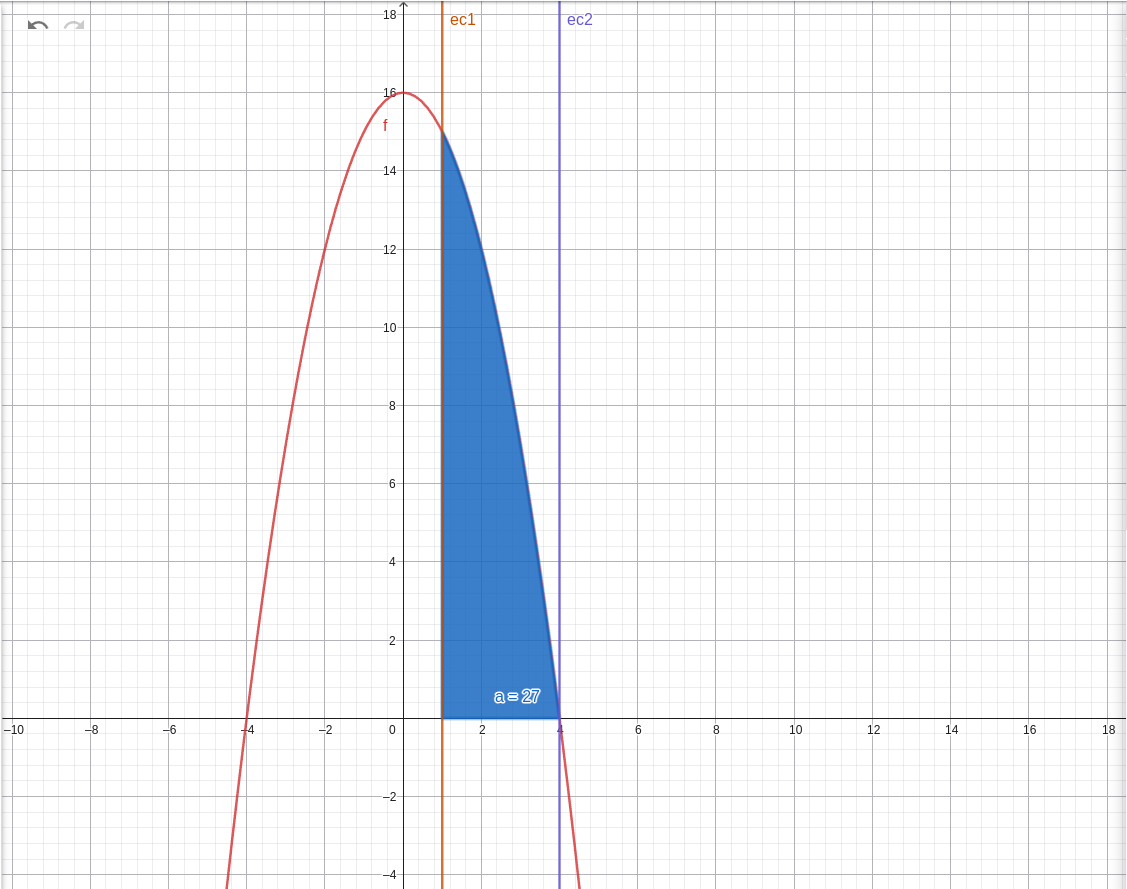
\includegraphics[width=0.5\textwidth]{Graficas/ejer9.png}
\end{center}
